\documentclass[arial,11pt]{article}
%\documentclass[11pt]{nih}
\usepackage[dvips]{graphicx}
\usepackage[colorlinks=true,linkcolor=black]{hyperref}
\usepackage{amssymb}
%\usepackage{graphicx}
%\usepackage{longtable}
\usepackage{epsfig}
%\usepackage{overcite}
\usepackage[usenames]{color}

\renewcommand{\rmdefault}{phv} % Arial
\renewcommand{\sfdefault}{phv} % Arial
\renewcommand{\thesection}{\Alph{section}}
\pagestyle{empty}

%\usepackage{times}
\usepackage{geometry}
%\geometry{tmargin=1in,bmargin=1.0in,lmargin=1in,rmargin=1in}
\geometry{tmargin=0.95in,bmargin=0.95in,lmargin=0.95in,rmargin=0.95in}
%\linespread{0.95} \interfootnotelinepenalty=10000

%%%%% editing helpers
\newcommand{\NeedRevision}[1]{\textcolor{red}{#1}}

\begin{document}

\begin{center}
\Large
{\bf Driving Biomedical Project 6:\\Molecular Networks in Diabetic Complications}
\normalsize
\end{center}

\begin{itemize}
%\item {\bf Funding status of the project:}  funded
\item {\bf Collaborating investigator:}  Kumar Sharma
\item {\bf Institution:} Division of Nephrology-Hypertension, Dept. Medicine, UCSD
\item {\bf Funded project:} 	Novel Paradigms in Diabetes Complications
\item {\bf Grant number:} 	1 DP3 DK094352 01   	
\item {\bf Project period:}   9/30/2011 to 8/31/2016,
\item {\bf Agency:}  NIDDK
\item {\bf TRD interactions:}  TRD3 (Spectral networks) and TRD8 (ProteoSAFe, MassIVE).
\end{itemize}

%  \begin{tabular}{rl}
%  Collaborating PI(s): & Kumar Sharma, M.D. \\
%  Institution: & University of California, San Diego \\
%  Funding: \\
%    NIH NIDDK & 1DP3DK094352-01, 9/30/2011 to 8/31/2016, PI Sharma
%  \end{tabular}
%\ \\\ \\
%{\bf TRD interactions: } TRD3 (Spectral networks) and TRD8 (ProteoSAFe/MassIVE).
%*******************************************
\section{Significance}
%*******************************************

%(1) Significance:
% address the importance as an impetus for TR&D of the biomedical research problem that will form the basis of the DBP;
% challenges inherent in this research problem that will drive TR&D;
% appropriateness of the DBP as a test-bed for technology being developed in the BTRC.

The understanding of the basic mechanism of cell dysfunction in response to diabetes is central to developing effective methods to prevent, diagnose, monitor and treat the complications of diabetes. Data generated by the Sharma laboratory from animal studies and humans challenges the dogma that elevated glucose levels leads to excess mitochondrial activity and excess production of mitochondrial superoxide anions. The consequent new hypothesis is that elevated blood glucose levels leads to an inhibition of mitochondrial function and synthesis and subsequent inflammation and fibrosis. If true, this characteristic response should be detectable in patients and animal models of diabetic kidney disease. It it likely that the degree of inhibition of mitochondrial function and mitogenesis will be the basis for future impaired reduction of glomerular filtration rate, a key function of the kidney cyto-architecture. This project focuses on proving this concept in patients with type 1 and type 2 diabetes and progressive kidney disease and in animal models of type 1 diabetes. By demonstrating the validity of this pathway and assessing new tools to monitor this pathway in humans, the data will significantly advance our understanding of diabetic complications and potentially alter the course of pharmaceutical approaches to treat diabetic complications~\cite{decleves10}.

Mitochondria are at the heart of the cellular decision tree for energy sensing and have adapted to the constant changes in the availability of nutrients in the environment. Mitochondria are also central players in the determination of cell death and survival and for tuning metabolism in tissue-specific ways for optimal organ function. Whereas the response of mitochondria to states of energy deficits are well understood the response of the mitochondria and the cell to caloric excess is unclear. The accepted theory to explain why humans develop diabetic complications is that excess calories are processed via mitochondria resulting in excess production of superoxide anion radical via the electron transfer chain 1. The resulting accumulation of superoxide within the mitochondria would then mediate downstream pathways related to cell dysfunction. However, the exciting new data generated from animal imaging demonstrates a completely opposite set of conclusions! There is actually a dramatic reduction of intracellular superoxide in response to hyperglycemia in the kidney following onset of diabetes. This project will test the hypothesis that reduced mitochondrial function in patients with type1 and type 2 diabetes and kidney disease predicts the rate of decline in renal function, that epigenetic changes of \mbox{PGC1$\alpha$} promoter methylation is increased in patients with type 1 diabetes and kidney disease, and that these changes are reflective of underlying renal function in mouse models of diabetic kidney disease.

%*******************************************
\section{Innovation}
%*******************************************

%(2) Innovation: Describe the innovations and technological advances that will result from the DBP interaction with Center TR&D and their implications beyond this project.

Having critically examined the accepted theory of diabetic complications using a novel in vivo approach to chart the time course of superoxide production in diabetic complications, the Sharma laboratory determined that the data was diametrically opposite to what was expected based on the standard Brownlee paradigm - there was a reduction in superoxide production despite evidence of early injury to the diabetic kidney (glomerular hypertrophy and albuminuria). Thus the data demonstrated provocative evidence that mitochondrial superoxide production was suppressed in the diabetic mice and may not play a major role in complications. However there was no prevailing theory to explain the data. The Sharma laboratory has developed a new evolutionary-based and physiologic theory to understand the data generated and to predict downstream consequences related to the development of inflammation and fibrosis. This project breaks with the prevailing and orthodox view that mitochondrial superoxide anions are the direct cause of cell and organ dysfunction in diabetes. The proposed experiments are directly relevant to novel biomarkers for diabetic kidney disease by applying novel methods to understand the urine metabolome and epigenome in humans with type 1 diabetes. The Sharma laboratory routinely uses GC-MS and LC-MS/MS to primary and secondary in human (and veterinary) biofluids. The available equipment includes HPLC systems, two automated amino acid analyzers, two GC-MS systems, three tandem LC-MS/MS mass spectrometers, and two hybrid quadrupole-time of flight instruments at the UCSD Biomolecular Mass Spectrometry Facility: an AB/Sciex QTrap 5500 LC/MS/MS system and an AB/Sciex TripleTOF 5600 mass spectrometer, a tandem quadrupole time of flight (QTOF) instrument. These will be used to perform comprehensive targeted and untargeted analyses of primary and secondary metabolites in urine samples in the FinnDiane and CRIC cohorts.

The detailed characterization of metabolic profiles in diabetes and kidney disease requires that the targeted approach be complemented by an untargeted ``discovery'' approach to assess the occurrence of unexpected or unidentified metabolites with high expression and/or correlation with disease profile. However, the identification of novel metabolites in urine and kidney tissue (i.e., when the molecule is not cataloged in existing databases) is currently a largely unaddressed challenge. In collaboration with CCMS, the untargeted MS/MS data collected in this DBP will drive the development of spectral matching algorithms for primary and secondary metabolites by searching against standard libraries (e.g., NIST, Metlin, MassBank, etc.) and by constructing and searching a reusable Kidney Atlas spectral library from patients with diabetes types 1/2 and mouse models of human disease (TRD3). In addition, molecular spectral networks analysis~\cite{watrous12,moree12} will also be used to find unexpected variants of known molecules and to help guide the follow up analysis of unidentified molecules found in diabetic vs non-diabetic kidney samples (TRD3). Finally, the multi-stage algorithmic workflows and the volume of data produced in this DBP will also drive the need for ProteoSAFe/MassIVE developments for primary and secondary metabolites (TRD8).

%*******************************************
\section{Approach}
%*******************************************

%(3) Approach: Describe methods and procedures to be used, emphasizing the relationship between the DBP and BTRC personnel and technologies, rationale for the proposed approach to the problem and impact of the expertise of the BTRC investigators and technology on the project.

The prevailing theory to explain the complications of type 1 diabetes is based upon the idea that exposure to excess glucose will set off a cascade of deleterious events, initially driven by over-production of mitochondrial superoxide anions. In contrast, this project hypothesizes that mitochondrial function and mitochondrial superoxide anion production is shut down in response to exposure to excess glucose. This effect, termed the Crabtree effect, if persistent will lead to Warburg metabolism which is closely tied to production of disease-promoting pro-fibrotic and inflammatory molecules.
The proposed studies will test this hypothesis in patients with type 1 diabetes at the metabolomic and epigenetic level and in experimental systems to prove our hypothesis and establish the molecular mechanisms driving this course of events in the diabetic kidney. Metabolomic and epigenetic analyses of reduced mitochondrial function and biogenesis will be performed in urine samples from 2000 patients in the FinnDiane and CRIC cohorts. Reduced mitochondrial function will set off an inflammatory and pro-fibrotic cascade leading to progressive cell dysfunction and reduction in the glomerular filtration rate. They postulate that the pathogenetic mechanism mediating the shutdown of mitochondria in diabetes is via inhibition of \mbox{PGC1$\alpha$}. The role of this pathway will be tested in mouse models of diabetic kidney disease using novel mass spectrometry methods and cell specific deletion of \mbox{PGC1$\alpha$}.

{\em Human urine metabolomics.} Urine metabolomic profiles in patients with type 1 and type 2 diabetes will be correlated with decline in kidney function. Preliminary results identified a panel of urine metabolites that reflect abnormal mitochondrial metabolism and are reduced in individuals with diabetic kidney disease. Urine samples from 1000 patients with type 1 diabetes in the FinnDiane study and 1000 patients with type 2 diabetes in the CRIC study will be assessed. The metabolomic profile will be correlated with future decline in kidney function over 6 years of follow-up. This will test the hypothesis that urine metabolite levels are an indication of renal cell dysfunction among individuals with diabetic chronic kidney disease and will be associated with the rate of decline of kidney function, independent of baseline eGFR, urine albumin to creatinine ratio, or other established risk factors for longitudinal decline in eGFR.

{\em Experimental animals metabolomics mass spectrometry and epigenomics.} This project will employ a series of animal studies to demonstrate the relationship between mitochondrial structure and function in progressive and non-progressive models of diabetic kidney disease in mice (Akita Bl6J and F1 cross of Bl6 and DBA/2). A series of imaging and biochemical studies will determine mitochondrial superoxide anion and mitochondrial function in early and established diabetes. Using \mbox{PGC1$\alpha$} floxed mice this project will determine the causal role of \mbox{PGC1$\alpha$} inhibition on glomerular mitogenesis and in the initiation and progression of diabetic kidney disease. Whole tissue metabolomics and whole genome methylation studies in kidney tissue and urine during the development of diabetic kidney disease will establish the relation between urine markers and renal disease. % Using a systems biology approach we will then demonstrate novel biomarkers that closely reflect and track renal mitochondrial status at the metabolomic and epigenetic level.

\begin{figure}[ht!]
%  \vspace{-20mm}
    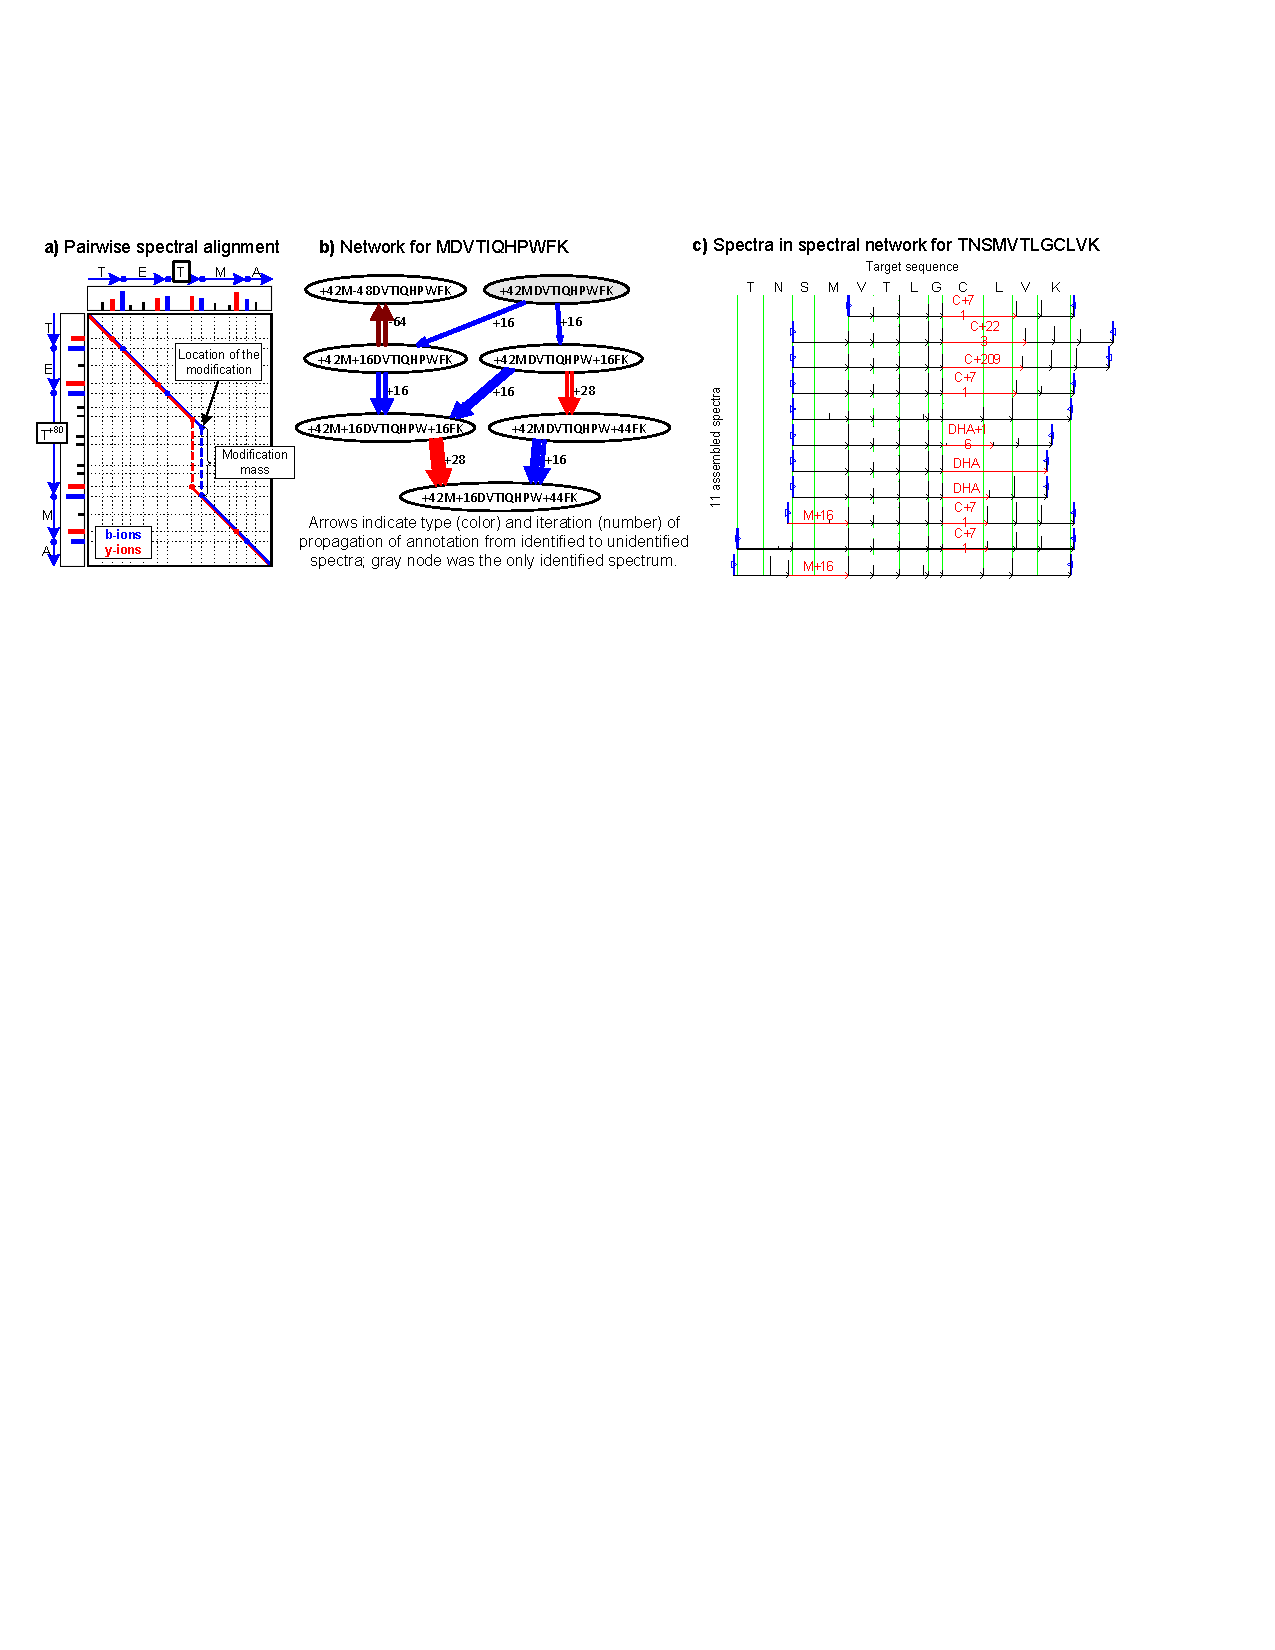
\includegraphics[width=\textwidth]{figures/figSpecNets.pdf}
%    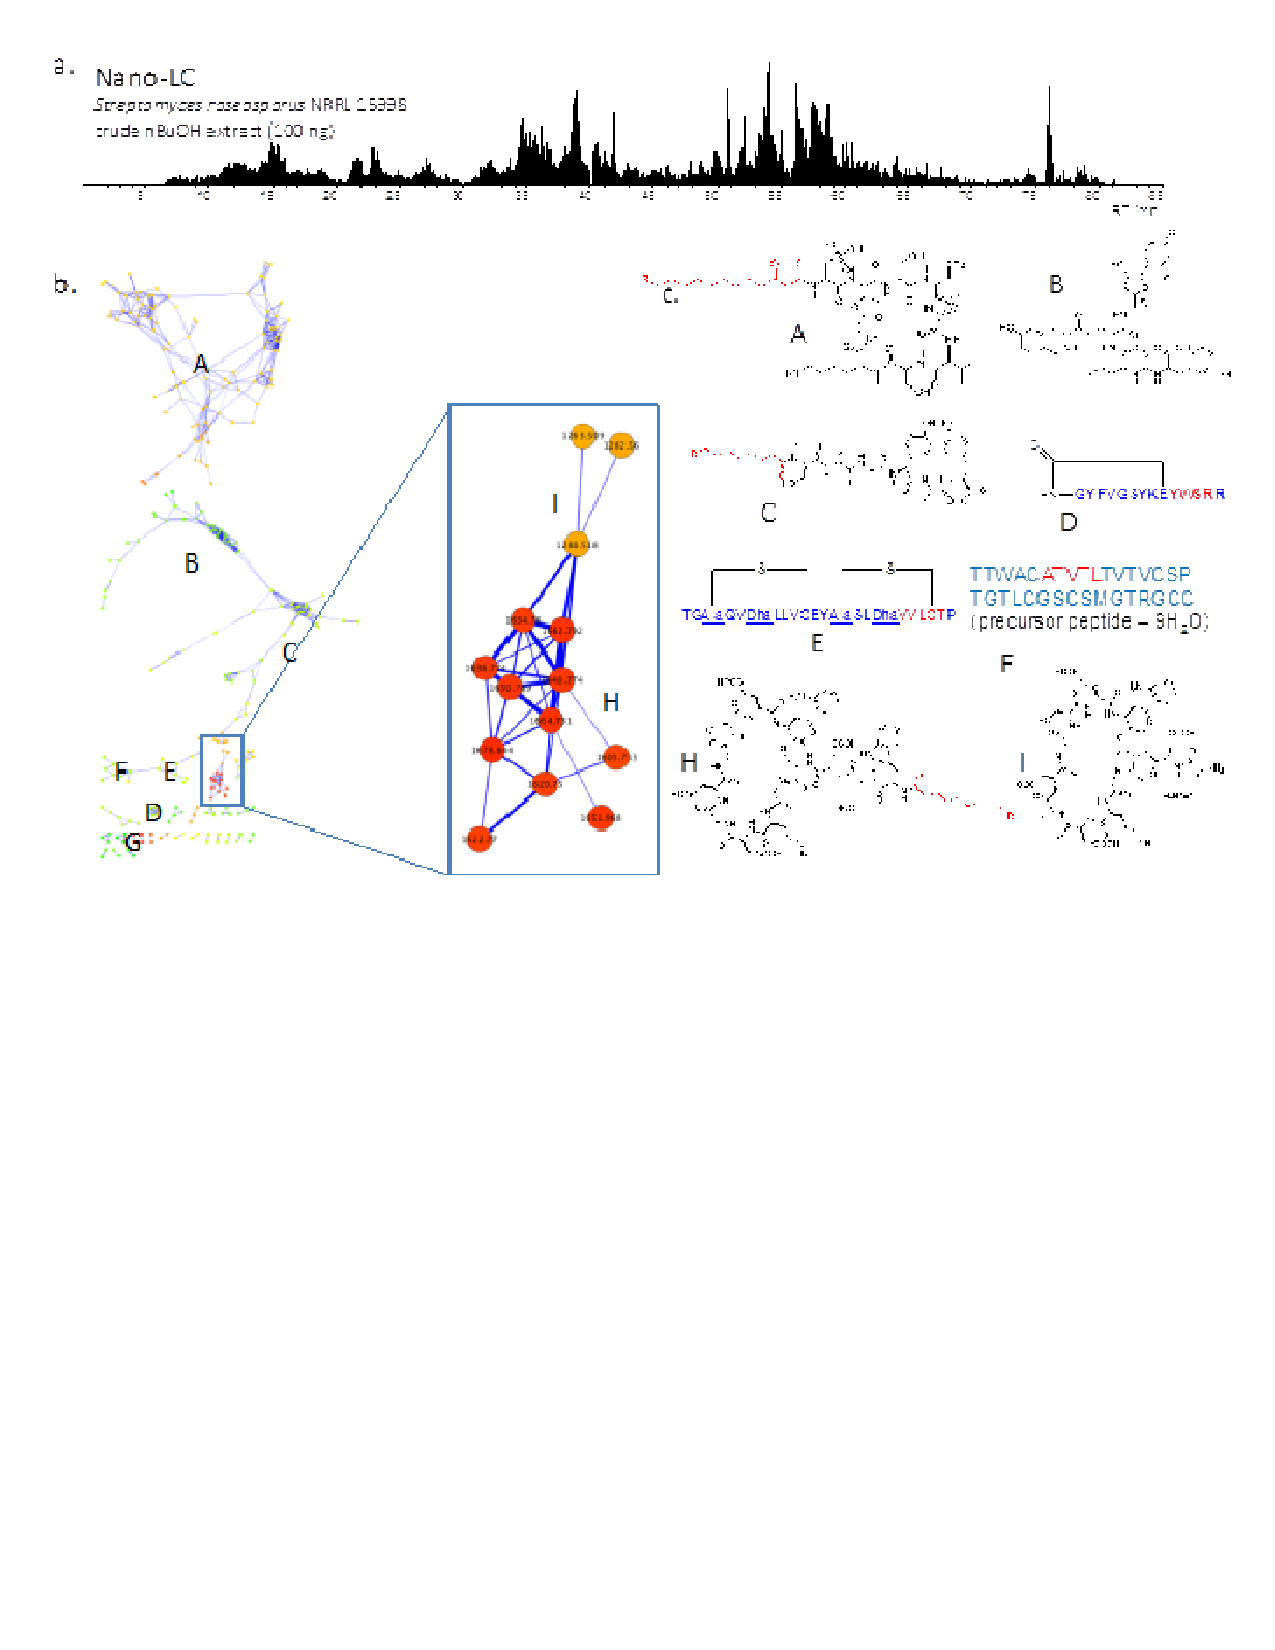
\includegraphics{figures/figApproach.png}
  \caption{{\bf Enabling untargeted metabolomics discovery while maintaining the
accuracy of quantification from targeted analysis.} (a) Untargeted mass spectrometry analysis of 20 isotopic standards spiked into depleted serum samples. Separate standard ratios obtained using constant concentrations of isotopic standards and a range of unlabeled standards spanning physiological ranges. % Quantification of organic acids from the same standard curve samples;
Left: (negative ionization, PFP column), Right: (positive ionization, SM-C18 column). Each curve had $\geq 6$ points, but some regression lines here were truncated to facilitate display. (b) Molecular spectral network revealing MS/MS spectral similarities among spectra of acetyl-(204.12), propiony-(218.14), isobutyryl-(232.16), isovaleryl-(246.17), octanoyl-(288.22), palmitoyl-(400.34) carnitine; every network node represents a different spectrum and edges represent significant spectral similarity. Spectral networks can be constructed without knowledge of metabolite identity and will
be used to facilitate annotation of unidentified variants. For example, if the annotation of octanoylcarnitine (288.22) was not known then it would be easier to interpret its spectrum using the knowledge that it is very similar to the spectra for the other acylcarnitines, and most similar to the other extended straight-chain species, palmitoylcarnitine (400.34).}
  \label{fig.dbp.sharma.molnets}
\end{figure}

%Features of interest from untargeted data sets are then searched for in databases such as HMDB and Metlin for both accurate mass and ms/ms matches. Significant progress has been made over the years to build these libraries m but a large number of metabolites are still either not catalogued in the databases or do not have ms/ms spectra available.
%
As a complement to targeted metabolomics studies the Sharma laboratory has developed a hybrid method that exploits the unique instrumentation characteristics of the AB/Sciex 5600 QqQ/ToF mass spectrometer.  Calibration curves have been determined for a growing number of compounds (presently 87) using a "semi-targeted" workflow \-- untargeted data acquisition with quantification enabled by addition of stable isotopes. This allowed for the quantification of a large number of metabolites, while also searching for other unanticipated metabolites within the same workflow.  In targeted analysis, the classification and visualization of results is extended by multivariate analysis and hierarchical cluster analysis~\cite{sumner07}. In untargeted analysis, MetAlign~\cite{sumner07} and XCMS~\cite{benton08} are used to smooth and align peaks across datasets. This analysis is also complemented with the proprietary software Multiquant for accurate absolute quantification and Markerview for efficient untargeted metabolomic data alignment and statistical analysis. This workflow has already been tested on a variety of samples (plasma, urine, and bloodspots) from control individuals at different times over weeks, and can be used to objectively gauge diurnal variation and the effects of feeding and fasting.
%
The choice between targeted and untargeted analysis will principally depend upon the specific study.

In collaboration with CCMS, this DBP will drive the construction of a Kidney Atlas of all MS/MS spectra of identified and unidentified urine metabolites in patients with diabetes type 1 (FinnDiane study) and type 2 (CRIC study), in addition to kidney tissue metabolites from mouse models of kidney disease. Automated identification of metabolite MS/MS spectra acquired in untargeted mode will be achieved by 1) using modification-tolerant search against the NIST spectral library and the annotated portion of the Kidney Atlas library of reference spectra (TRD3) and 2) by constructing molecular spectral networks of related metabolites (e.g., acetylcarnitine, propionylcarnitine, isobutyrylcarnitine, etc). The Kidney Atlas spectral library will be initialized with reference spectra for all standard metabolites used in targeted experiments and will be extended by importing all high-quality searchable reference spectra from publicly available resources. In addition to supporting automated identification of untargeted MS/MS spectra by matching against reference spectra, the Kidney Atlas will also include spectra of unidentified metabolites discovered in untargeted analysis. These unidentified spectra will be cross-referenced across all untargeted runs such that a positive identification made in one mass spectrometry run will be automatically transferred to all other stored runs where the metabolite was previously unidentified (TRD8). Molecular spectral networks algorithms (TRD3) will be used to a) find spectra of unidentified compounds with significantly-similar fragmentation at 5ppm fragment mass accuracy and b) build a network showing MS/MS similarity relationships between unidentified compounds. In particular, molecular spectral networks will greatly facilitate the identification of related compounds by illustrating the relationships to known compounds. As illustrated in Figure~\ref{fig.dbp.sharma.molnets}, if the identity of palmitoylcarnitine would not have been known in advance, its spectral networks relationships to octanoylcarnitine, isovalerylcarnitine, etc. would have greatly facilitated its annotation. As novel compounds become identified, their reference MS/MS spectra will be added to the Kidney Atlas to enable fully-automate identification for all future searches.

\paragraph{Impact of the expertise of the CCMS investigators on DBP.} Drs. Bandeira and Pevzner were the original proponents of the spectral networks paradigm for analysis of peptide MS/MS spectra~\cite{bandeira04,bandeira07pnas,guthals12specnets} and have since extended and applied it to analysis of post-translational modifications~\cite{gonzalez10,yang11} and de novo protein sequencing~\cite{bandeira07mcp,guthals12metasps}. Dr. Bandeira has also proposed novel methods for spectral library search~\cite{wang10} and recently further extended the spectral networks paradigm to construct molecular spectral networks for any type of molecules suitable for analysis with tandem mass spectrometry, which was demonstrated on the analysis of primary and secondary metabolites in microbial interactions~\cite{watrous12,moree12}. Dr. Bandeira also led the development of the ProteoSAFe platform which already enabled the analysis of over 1 billion spectra and thus has the required expertise to implement, search and distribute the proposed Kidney Atlas.


%%**************************************************************************************
%% ------------------------------------------------------------------------------------
%\section{Technology Research and Development projects (TR\&Ds)}
%% ------------------------------------------------------------------------------------
%%**************************************************************************************
%
%This DBP will drive and substantially benefit from the proposed CCMS research and development on $i)$ spectral libraries and networks algorithms and statistics (TRD3) and $ii)$ natural products searching and de novo sequencing algorithms (TRD2). In addition, the likely complexity of the resulting software and the expected volume of data to be processed will further drive the need for the proposed ProteoSAFe developments and MassIVE resources proposed here (TRD8).

% For all 3 aims

%\bibliographystyle{plain}
\bibliographystyle{plain}
\bibliography{../../bibtex/msms,../../bibtex/bandeiraLab,../../bibtex/immunology,sharma}
\end{document}
